%!TEX root = ../template.tex
%%%%%%%%%%%%%%%%%%%%%%%%%%%%%%%%%%%%%%%%%%%%%%%%%%%%%%%%%%%%%%%%%%%%
%% chapter3.tex
%% NOVA thesis document file
%%
%% Chapter with a short latex tutorial and examples
%%%%%%%%%%%%%%%%%%%%%%%%%%%%%%%%%%%%%%%%%%%%%%%%%%%%%%%%%%%%%%%%%%%%

\typeout{NT FILE chapter3.tex}%

\makeatletter
\newcommand{\ntifpkgloaded}{%
  \@ifpackageloaded%
}
\makeatother


\chapter{Proposal}
\label{cha:Proposal}


This chapter presents the original \emph{thesis proposal} that guided the early stages of this work. It outlines the initial plan for developing an AI-driven tool to automate anomaly detection in Sanger sequencing workflows, including the overall vision, technical approach, and model choices that informed the first phase. The subsequent chapters (\S\ref{cha:Implementation}--\ref{cha:Evaluation}) document how the design evolved and why.

The goal of the proposed system was to improve the efficiency and accuracy of well verification in 96-well sequencing plates by reducing reliance on manual review. By leveraging machine learning techniques, the system was expected to automatically categorize DNA samples based on sequence similarity and associated metadata, enabling faster detection of contamination or sequencing errors.

The chapter begins with an overview of laboratory processes and data generation, then introduces the original architecture and preprocessing pipeline (e.g., DBSCAN + Random Forest). This proposal served as the conceptual foundation for later development.

\section{Laboratory Processes}
\label{sec:laboratory}

The laboratory processes described here are central to the generation of the data used in this work. These processes involve the handling of DNA samples, their preparation for sequencing, and the subsequent analysis of the results.

\subsection{Sample Preparation and Processing}
The laboratory workflow begins with the reception of DNA samples from various clients. These samples are organized into 96-well PCR plates, where each well is identified by a unique coordinate system: letters A to H for the rows and numbers 1 to 12 for the columns (Figure \ref{fig:96_well_plate}). This organization ensures traceability and efficient handling of multiple samples simultaneously. Samples from the same client are grouped together in neighboring wells, although not all wells need to be occupied for sequencing to proceed.
\begin{figure}[H]
  \centering
  \includegraphics[width=0.8\textwidth]{96plate.png}
  \caption{A 96-well PCR plate.}
  \label{fig:96_well_plate}
\end{figure}


\begin{figure}[H]
  \centering
  \includegraphics[width=0.8\textwidth]{platecoords.png}
  \caption{Structure and Organization of each PCR plate.}
  \label{fig:platecoords}
\end{figure}

Upon receipt, some samples require human intervention to prepare them for sequencing. For instance, samples with uneven DNA concentrations must be normalized to ensure consistent sequencing quality. Additionally, samples that do not include a primer must have the appropriate primer added by laboratory staff. These steps are critical to ensure the accuracy and reliability of the sequencing results. Each plate also contains 1 well reserved solely for quality control, named control well.

Once prepared, these plates are then loaded into a thermocycler, which includes the steps of DNA denaturation, primer annealing, and extension with fluorescently labeled dideoxynucleotides. Afterwards the electrophoresis is performed on the ABI3730xl sequencer. The ABI3730xl sequencer then generates raw data files containing fluorescence intensity readings, which are subsequently basecalled to produce DNA sequences.


\subsection{The ABI3730xl DNA Sequencer}
The ABI3730xl DNA sequencer is a high-throughput instrument widely used in genomics for Sanger sequencing. It automates the electrophoresis and fluorescence detection steps, corresponding to steps 3 and 4 of the Sanger sequencing process (Figure \ref{fig:sanger_steps}), allowing for the simultaneous processing of 96-well plates in a single run \cite{smith_capillary_sequencing,abi3730xl_overview}. By leveraging this technology, laboratories can achieve precise and efficient DNA sequencing. 
\begin{figure}[h]
\centering
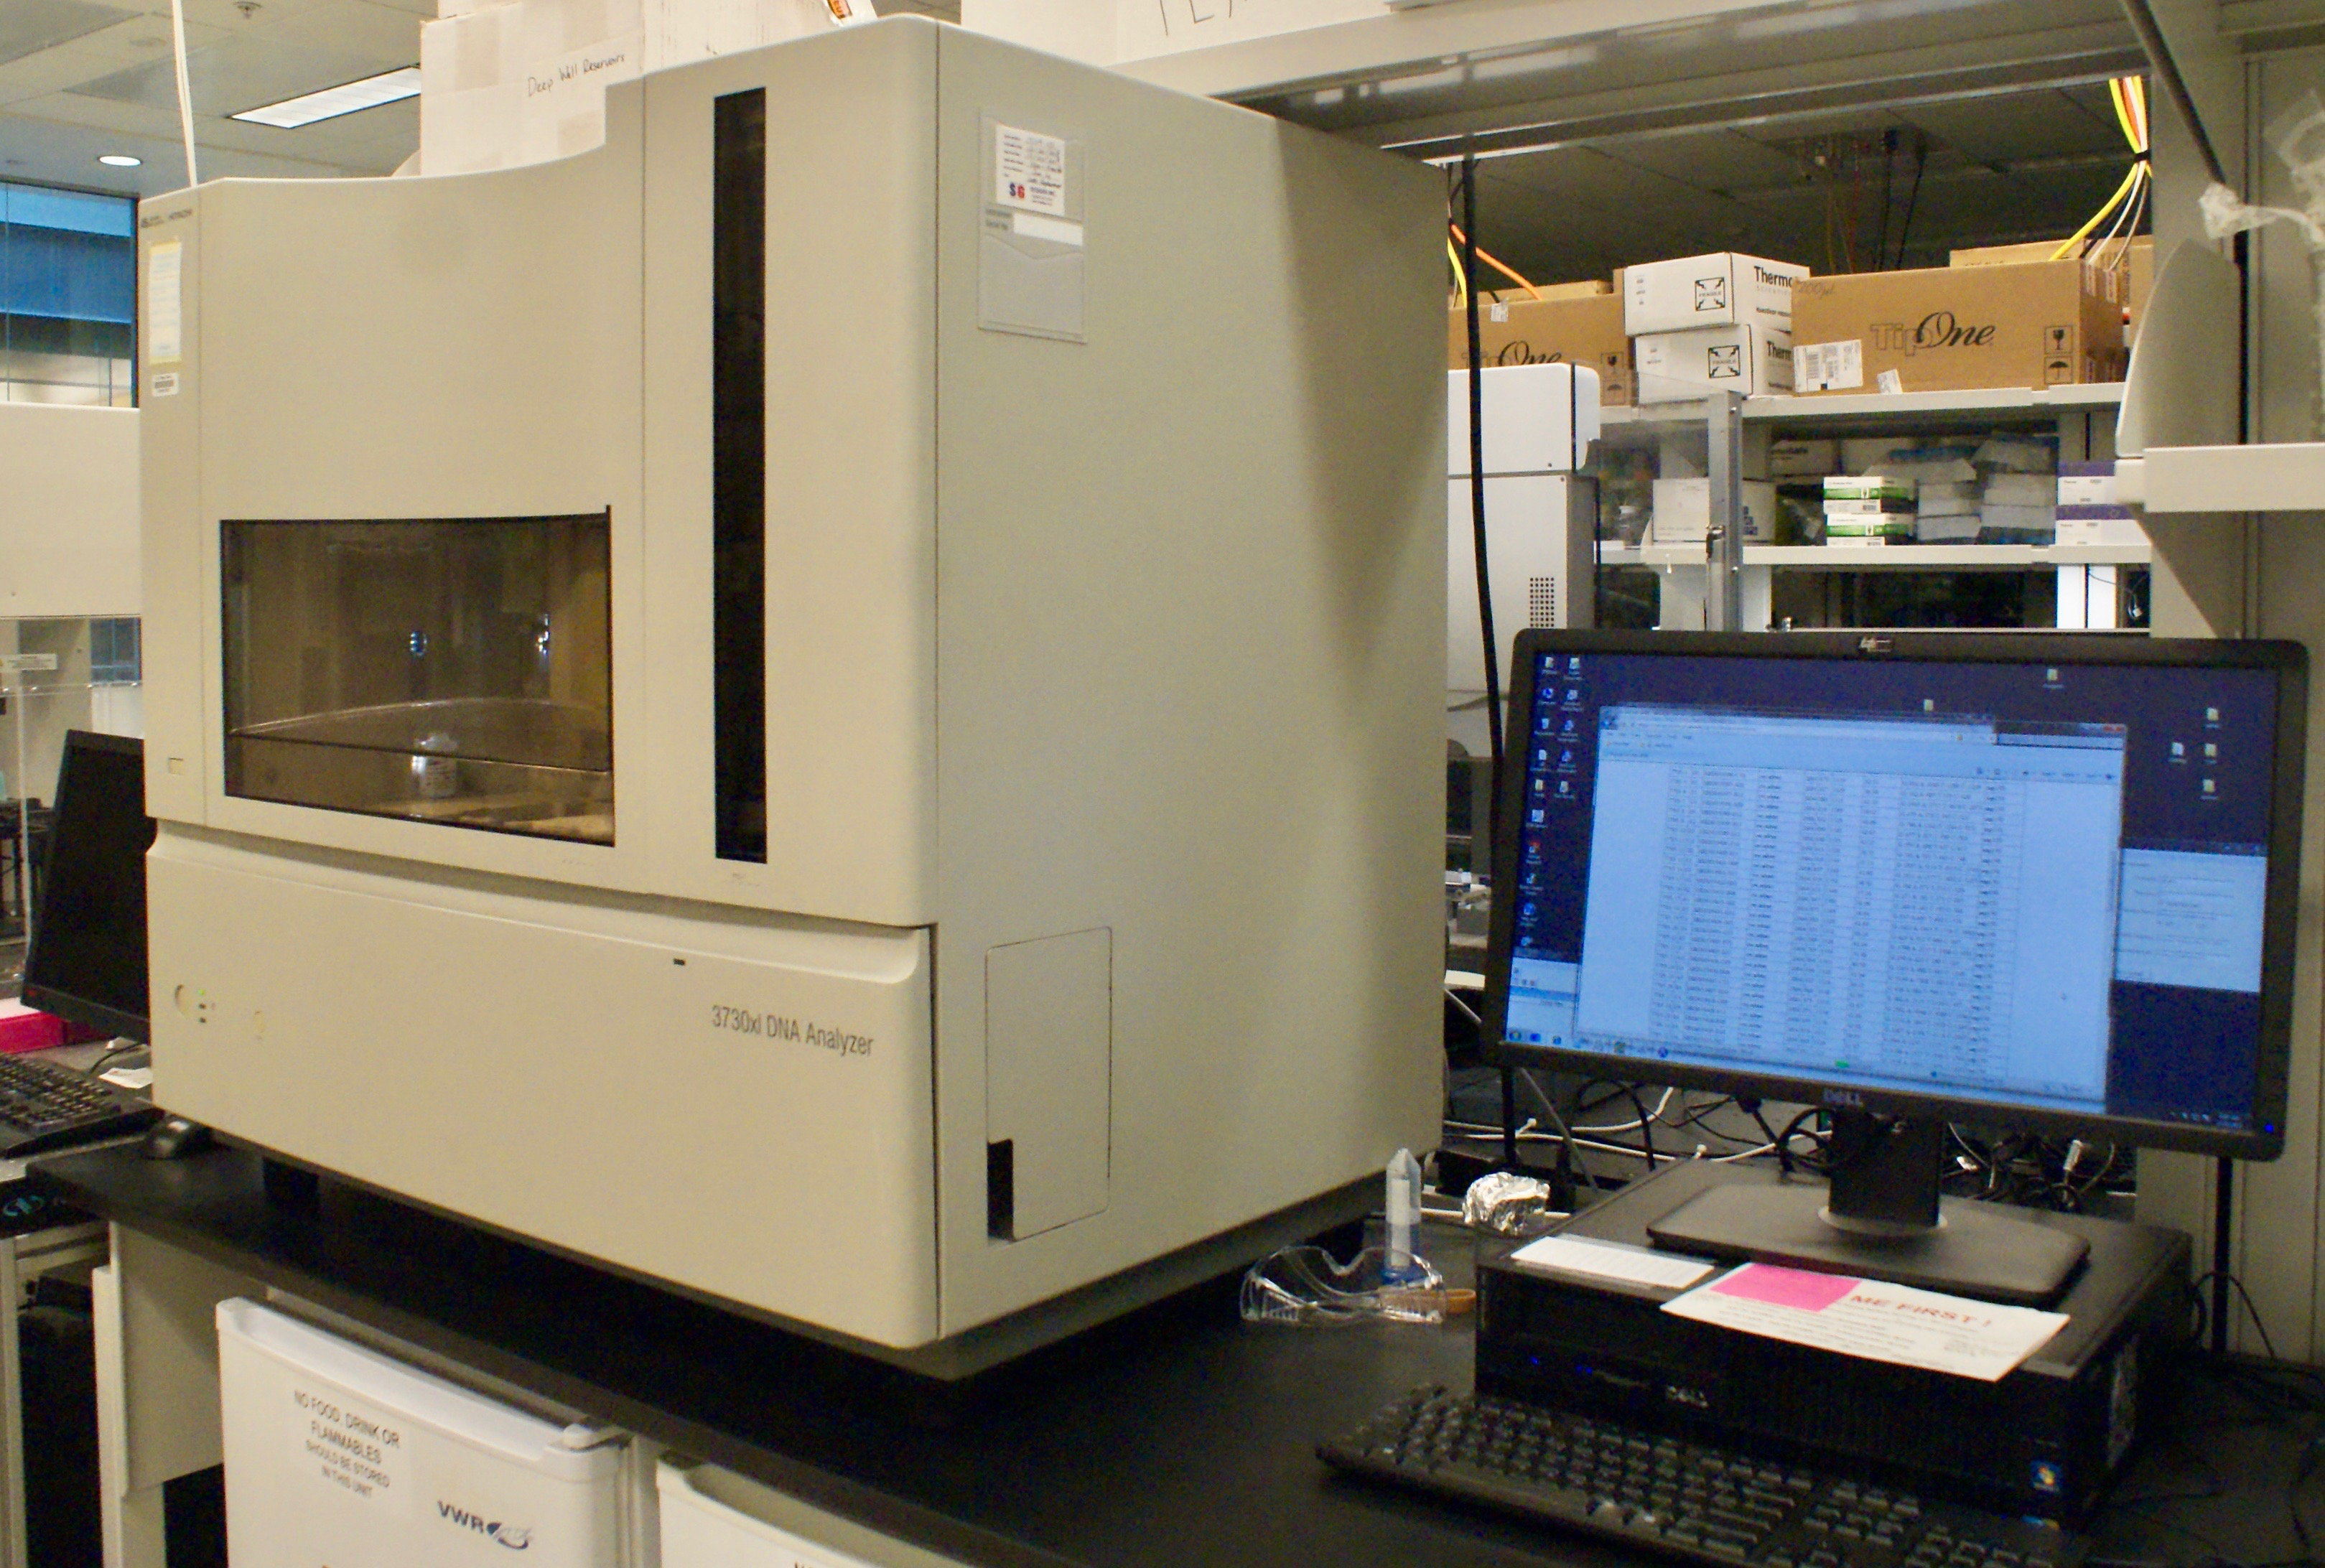
\includegraphics[width=0.7\textwidth]{abi_3730xl_closed.png}
\caption{A closed ABI3730xl capillary electrophoresis DNA analyzer.}
\label{fig:abi_3730xl_closed}
\end{figure}

\begin{figure}[h]
\centering
\includegraphics[width=0.7\textwidth]{abi_3730xl_opened.png}
\caption{An opened ABI3730xl capillary electrophoresis DNA analyzer.}
\label{fig:abi_3730xl_opened}
\end{figure}

\subsection{Data Generation}

The effectiveness of any artificial intelligence model relies heavily on the quality and structure of the available data. In this work, the data originates from customer samples sequenced using the ABI3730xl DNA sequencer. Each well in a 96-well PCR plate generates multiple files, including raw fluorescence data, processed DNA sequences, and quality metrics. With each plate containing 96 wells and each well producing 6 distinct files, a single plate yields 576 files. Over time, as multiple plates are processed daily, this results in millions of files, forming a robust dataset for analysis.
The primary file types considered in this work include:

\begin{itemize}
  \item \textbf{Ab1 File}: Contains intensity readings for each of the four fluorescent dyes (A, T, C, G) used in Sanger sequencing, resulting in fluorescent traces. This file is optimized for long sequences (more than 500 bases).
  \item \textbf{Phd1 File}: Contains the DNA sequence derived from the fluorescence traces, along with quality scores and scan numbers.
  \item \textbf{Scf File}: Similar to .ab1 files, .scf files include quality information about the base calls, the chromatogram (also called the electropherogram), and the DNA sequence.
  \item \textbf{Seq File}: A plain text file containing the DNA sequence.
  \item \textbf{Qual File}: Includes the quality scores of each base in the DNA sequence.
  \item \textbf{Qualtrace File}: Contains additional information about the sequencing process, such as PeakStart, DyeSignal, Noise, and Spacing.
\end{itemize}

These files adhere to a strict naming convention: \textbf{ReactionID\_Pos\_DNAID+PrimerID}. 
For example, the file name \texttt{2338715\_A1\_AA8117+Clon\_2+ORB501} can be broken down as follows:
\begin{itemize}
  \item \texttt{2338715}: The unique reaction ID.
  \item \texttt{A1}: The position of the well in the plate (row A, column 1).
  \item \texttt{AA8117+Clon\_2}: The DNA ID, identifying the specific DNA sample.
  \item \texttt{ORB501}: The primer ID, which is optional as some customers provide samples with primers already included.
\end{itemize}
Thus, 6 files are generated for this specific well: 
\begin{itemize}
  \item \texttt{2338715\_A1\_AA8117+Clon\_2+ORB501.ab1}
  \item \texttt{2338715\_A1\_AA8117+Clon\_2+ORB501.phd.1}
  \item \texttt{2338715\_A1\_AA8117+Clon\_2+ORB501.scf}
  \item \texttt{2338715\_A1\_AA8117+Clon\_2+ORB501.seq}
  \item \texttt{2338715\_A1\_AA8117+Clon\_2+ORB501.qual}
  \item \texttt{2338715\_A1\_AA8117+Clon\_2+ORB501.qualtrace}
\end{itemize}

Other relevant and important information about each plate well, such as the associated \textbf{Client's Name}, \textbf{Sequence Length}, \textbf{Primer DNA Sequence} (If applied by the laboratory staff), and the \textbf{Control Well Status} is also available.  
\newline
It is also important to note that while DNA sequences are primarily composed of the four canonical bases: adenine (A), thymine (T), cytosine (C), and guanine (G), some sequences contain additional IUPAC ambiguity codes such as \texttt{N} (any base) or \texttt{Y} (C or T). These ambiguous bases typically arise from basecalling uncertainty in low-quality signal regions. Their presence has implications for downstream processing, especially for sequence encoding in machine learning models, which would need to be addressed during downstream sequence encoding.
\newline
\subsection{Manual Analysis}

After the data is generated, the laboratory staff manually handles quality checks on each plate individually, particularly for identifying possible fluorescence contamination and mismatches in sequencing results. This is a lengthy and thorough process that currently induces a bottleneck in the laboratory workflow. The main steps for quarantining wells are as follows:

\begin{itemize}
  \item \textbf{1. Control Well Check}: The laboratory staff begins by checking the \texttt{control\_well} for each plate. If the control well's \texttt{ok\_flag} is \texttt{NOT OK}, the entire plate is quarantined, as this indicates a problem with the sequencing process. If the control well passes the check, the process moves to the next step.
  \item \textbf{2. Sequence Clustering}: The sequencing software extracts the \texttt{ab1} files from each well (96 wells per plate) and clusters the sequences based on a minimum similarity of 66\%. This clustering is performed to group together DNA samples that are likely to belong to the same biological entity. Each cluster represents a set of related DNA sequences.
  \item \textbf{3. Cluster Verification}: The next step involves verifying these clusters for potential contamination or sequencing errors. Laboratory staff checks for two main conditions:
    \begin{itemize}
      \item \textit{Similar Sequences from Different Clients}: If samples from different clients have very similar DNA sequences, it may suggest fluorescence contamination, triggering a quarantine for further investigation.
      \item \textit{Same Primers with Different Sequences}: If different primers are associated with very similar DNA sequences, this could indicate contamination and thus requires quarantining.
    \end{itemize}
  \item \textbf{4. Forward and Reverse Sequence Matching}: DNA samples are analyzed based on forward and reverse sequencing. If a single base mismatch is detected in the same DNA sample (with matching \texttt{DNAID} and \texttt{primer\_id}), it is flagged for quarantine. In the case where a sample is processed with different primers, a variation in sequence is expected.
\end{itemize}
Sometimes certain samples do not appear to be contaminated, but the overall suspicion of such, or the poor quality presented, is enough to justify a quarantine, due to the importance of delivering accurate results.
After the anomalies are quarantined, these possibly contaminated samples are re-sequenced for an attempt at acquiring higher quality and accuracy, while the remaining samples are delivered to the client.

\paragraph{Labeled Anomalies:} Although anomalies are not registered automatically in the laboratory's database, a small set of manually verified anomalies was made available upon request. Due to the rarity of confirmed contamination or sequencing errors in practice, the laboratory only identified \textbf{four plates} with known anomalies during the course of the data collection of this thesis. These labeled plates were used for evaluating the performance of the proposed models against the laboratory’s ground truth. This scarcity of labeled anomalies further justified the adoption of machine learning strategies throughout the project.

\begin{table}[H]
\centering
\caption{Manual workflow vs. proposed automation (proposal phase).}
\label{tab:manual_to_auto}
\begin{tabular}{|p{5.2cm}|p{9cm}|}
\hline
\textbf{Manual Step} & \textbf{Proposed Automation (at proposal time)} \\ \hline
Control-well check & Rule: if control \texttt{NOT OK} $\Rightarrow$ quarantine entire plate. \\ \hline
Cluster sequences ($\geq$66\% similarity) & DBSCAN over k-mer vectors to form clusters; ignore outliers. \\ \hline
Different clients, very similar sequences & Cluster-level metadata checks: flag mixed-client clusters. \\ \hline
Different primers, very similar sequences & Cluster-level rule: flag unexpected primer–sequence similarity. \\ \hline
Forward vs. reverse mismatch (same DNAID) & Pairwise alignment and per-sample rules; escalate on single-base mismatch. \\ \hline
\end{tabular}
\end{table}

\section{Initial Proposed Architecture}
\label{sec:initial_architecture}

Grounded in the laboratory workflow and data described above, we formulated an initial theoretical approach to automate plate-level quality control. The initial system design aimed to automate the manual verification of 96-well Sanger sequencing plates using artificial intelligence. The proposed approach focused on replicating the laboratory’s reasoning process using a combination of clustering techniques and anomaly detection models. The intention was to streamline the pipeline from data ingestion to anomaly flagging, leveraging both sequence similarity and metadata.

This section presents the architecture that was initially envisioned, including the database schema, preprocessing pipeline, and the selection of machine learning models. This intial design served as a conceptual and experimental foundation.


\subsection{Database Structure}

At proposal time we defined a \emph{logical per-well table schema} independent of storage technology. A NoSQL plate-as-document option was briefly considered but deferred. The essential idea was to model, for each plate, a single row per well aggregating identifiers, sequence text, quality metrics, and run metadata. The concrete mechanism to populate this schema (a unified per-plate export) was implemented later during the development phase (see Chapter~\ref{cha:Implementation}).

\paragraph{Original Proposed Schema:}  
At the proposal stage, the following schema was envisioned based on assumptions about data availability and early exploration of STAB VIDA’s sequencing workflow. The table included planned fields ranging from raw fluorescence traces to primer sequences and purification metadata.

\begin{table}[H]
  \centering
  \begin{tabular}{|l|l|p{8cm}|}
    \hline
    \textbf{Column Name} & \textbf{Data Type} & \textbf{Description} \\ \hline
    \texttt{Plate\_ID} & String & Unique identifier for each 96-well PCR plate. \\ \hline
    \texttt{Well\_POS} & String & Unique identifier for each well position (e.g., A1, B2). \\ \hline
    \texttt{Reaction\_ID} & String & Unique identifier for the reaction associated with the well. \\ \hline
    \texttt{DNA\_ID} & String & Identifier for the DNA sample. \\ \hline
    \texttt{Primer\_ID} & String & Identifier for the primer used (if applicable). \\ \hline
    \texttt{Client\_Name} & String & Name of the client associated with the sample. \\ \hline
    \texttt{Control\_Well\_Status} & String & Status of the control well (e.g., "OK" or "Quarantine"). \\ \hline
    \texttt{DNA\_Sequence} & Text & The DNA sequence derived from the `.seq` or `.phd.1` file. \\ \hline
    \texttt{Base\_Length} & Integer & The total number of bases of the DNA sequence. \\ \hline
    \texttt{Quality\_Scores} & Text & Quality scores for each base in the sequence (from `.qual` or `.phd.1` files). \\ \hline
    \texttt{Fluorescence\_Traces} & Text & Fluorescence intensity readings (from `.ab1` or `.scf` files). \\ \hline
    \texttt{PCR\_Size} & Integer & Size of the PCR product. \\ \hline
    \texttt{Purification\_Details} & Text & Information about the purification process. \\ \hline
    \texttt{Primer\_Sequence} & Text & Sequence of the primer used (if manually added by staff). \\ \hline
    \texttt{Date\_Processed} & Date & Date the plate was processed. \\ \hline
    \texttt{Anomaly\_Detected} & Integer & Although limited, some data is labeled with this flag. \\ \hline
  \end{tabular}
  \caption{Table Structure for Sequencing Data and Metadata.}
  \label{tab:unified_table}
\end{table}

This table structure ensured that all relevant information of each well derived from different generated files, is stored in a single organized row, simplifying data retrieval and analysis. It includes fields for plate and well identification, sequencing data, quality metrics, and metadata, making it suitable for both clustering and contamination detection tasks.

\paragraph{Operational dependency (proposal).}
At the time of the proposal, a unified per-plate export did not yet exist. We specified this as an implementation requirement; the company later delivered a backend export page that produced the input needed for this schema (cf. Chapter~\ref{cha:Implementation}).

\subsection{Data Preprocessing (Feature Engineering)}

To ensure optimal input quality for the AI-based model, multiple preprocessing steps are performed on the raw sequencing data. This includes sequence trimming, feature extraction, normalization of numerical features, and handling categorical/text-based attributes appropriately.

\subsubsection{Sequence Trimming}
Raw sequencing data contains noise, in the form of poor base quality, particularly at the start and end of sequences. At the beginning, this is primarily due to inefficient primer binding and weaker signal intensities as the primer binds and starts the reaction. At the end, the reduced availability of chain-terminating nucleotides (ddNTPs), declining polymerase efficiency, and signal saturation contribute to weaker and less accurate readings. \cite{sanger_method_original}

\begin{figure}[h]
  \centering
  \includegraphics[width=0.7\textwidth]{noise1.png}
  \caption{Visualization of noise in the beginning of the DNA sequence, using 4peaks.}
  \label{fig:noise1}
\end{figure}

\begin{figure}[h]
  \centering
  \includegraphics[width=0.7\textwidth]{noise2.png}
  \caption{Visualization of noise in the end of the DNA sequence, using 4peaks.}
  \label{fig:noise2}
\end{figure}

To improve downstream analysis, sequences are trimmed using the following criteria:

\begin{itemize}
    \item Bases are removed from the start and end of the sequence until \textbf{10 consecutive bases} have a \textbf{quality score} greater than 20.
    \item This threshold ensures high-quality regions are retained, as a quality score of 20 corresponds to a base-calling accuracy of 99\% \cite{quality_score_threshold}.
\end{itemize}

The trimmed sequences are then stored for subsequent steps.

\subsubsection{Sequence Encoding}
To represent DNA sequences in a numerical format suitable for clustering:
\begin{itemize}
    \item \textbf{k-mer Frequency Encoding}:
    \begin{itemize}
        \item Each DNA sequence is converted into a vector of k-mer frequencies.
        \item A k-mer size of 4 is chosen to balance specificity and computational efficiency, as tetramers provide sufficient resolution for pattern recognition \cite{kmer_size_choice}.
        \item For example, a 4-mer approach splits the sequence into overlapping subsequences of length 4 (tetramers) and counts their occurrences.
        \item This method captures local sequence patterns and is particularly useful for clustering algorithms like DBSCAN.
    \end{itemize}
\end{itemize}

\subsubsection{Normalization}
To ensure consistent scaling of features, while also ensuring numerical features contribute equally to the model:
\begin{itemize}
    \item \textbf{Sequence Feature Normalization}:
    \begin{itemize}
        \item The k-mer frequency vectors and the numerical features such as quality scores, sequence lengths, and other quantitative features, are normalized using \textbf{min-max scaling} or \textbf{z-score normalization} \cite{normalization_methods}.
        \item This ensures all features are on a similar scale, preventing any single feature from dominating the clustering process.
    \end{itemize}
\end{itemize}

\subsubsection{Dimensionality Reduction}
To handle the high dimensionality of k-mer frequency vectors:
\begin{itemize}
    \item \textbf{Principal Component Analysis (PCA)}:
    \begin{itemize}
        \item PCA is applied to reduce the dimensionality of the feature space while retaining the most significant variance.
        \item This step reduces computational complexity and mitigates the risk of overfitting.
        \item The number of principal components is selected based on the cumulative explained variance, retaining 95\% of the variance for example is a common threshold to balance complexity and information retention \cite{jolliffe2016}.
    \end{itemize}
\end{itemize}


\subsection{Model Selection \& Development}

The goal of the proposed AI-based tool is to fully automate the process currently performed manually by the laboratory staff. This involves categorizing DNA samples into wells based on their similarity and identifying anomalies that could indicate contamination, sequencing errors, or other irregularities. Since the proposed work is based on AI, there is a clear need to choose appropriate models for specific tasks. Given the complexity of the problem and the multiple steps involved in manual analysis---ranging from sequence clustering to anomaly detection---a \textbf{hybrid approach} is proposed to achieve both tasks. This approach leverages \textbf{two machine learning models}, one for clustering and another for anomaly detection inside these formed clusters:

\begin{itemize}
    \item \textbf{Unsupervised Clustering (DBSCAN)}: Groups DNA sequences based on similarity, mimicking the laboratory's manual clustering process without requiring labeled anomalies.
    \item \textbf{Supervised Classification (Random Forest)}: Detects anomalies using labeled data and features derived from clustering, enhancing detection accuracy.
\end{itemize}

Thus, a \textbf{structured pipeline} seems to be a good choice and starting point for streamlining the data from one model to another, combining the strengths of unsupervised and supervised learning to address the dual challenges of sequence similarity and anomaly detection.

\subsubsection{Unsupervised Learning for Clustering - DBSCAN}
Given the lack of cluster information data in the initial stages, unsupervised learning is particularly suitable for this task, as we first need to group samples that appear to be similar to each other together, indicating they are possibly from the same client. 
Unlike centroid-based methods like K-means, DBSCAN does not require predefined cluster numbers, making it adaptable to diverse datasets.
DBSCAN is used to group sequences into clusters based on their k-mer frequency representations. This unsupervised approach identifies natural groupings in the data, allowing for the detection of anomalies within clusters.

\begin{itemize}
    \item \textbf{Parameter Tuning}:
    \begin{itemize}
        \item The key parameters—\textit{eps} (maximum distance between samples in the same cluster) and \textit{min\_samples} (minimum number of samples in a cluster)—are optimized using grid search and silhouette score evaluation.
    \end{itemize}

    \item \textbf{Cluster Formation}:
    \begin{itemize}
        \item Sequences are grouped into clusters based on their similarity in k-mer frequency space.
        \item \textbf{Samples not assigned to any cluster} are ignored, as the focus is on detecting anomalies within clusters.
    \end{itemize}

    \item \textbf{Prediction}:
    \begin{itemize}
        \item The cluster labels (0, 1, etc.) now act as pseudo-labels for grouping similar samples in the following model.
        \item Outliers (-1) are ignored.
    \end{itemize}
\end{itemize}

\subsubsection{Semi-Supervised Learning for Anomaly Detection - Random Forest}
To leverage the limited labeled anomalies provided by the laboratory team, a semi-supervised learning approach is proposed. This combines the unsupervised clustering results from DBSCAN with a supervised classifier to identify samples that do not belong in their assigned clusters.

\begin{itemize}
    \item \textbf{Using DBSCAN's output with the labeled data available}:
    \begin{itemize}
        \item Manually labeled anomalies (from laboratory annotations) are combined with DBSCAN’s pseudo-labels to create a semi-supervised dataset for training.
    \end{itemize}

    \item \textbf{Classification with Random Forest}:
    \begin{itemize}
        \item A Random Forest classifier is trained on the labeled dataset due to its robustness and interpretability.
        \item Feature importance analysis is performed to identify which k-mers contribute most to detecting anomalies within clusters.
    \end{itemize}

    \item \textbf{Prediction}:
    \begin{itemize}
        \item The trained classifier predicts whether a sample belongs to its assigned cluster, flagging it as an anomaly if it does not.
        \item This provides automated quarantine recommendations for samples that are likely to be misassigned within clusters.
    \end{itemize}
\end{itemize}

\subsection{Evaluation (Planned)}
Clustering quality would be scored via silhouette/Davies–Bouldin; anomaly detection via precision, recall, F1, and confusion matrices. Thresholds would be tuned to prioritize recall (safety-first), as in this proposal stage, it was already understood that the laboratory team prioritized a higher percentage of a plate being flagged as an anomaly, given that all anomalies were successfully detected, rather than some anomalies managing to slip away detection due to a low percentage of flagged wells.

\subsection{Frameworks, Languages \& Tools}
The development and implementation of the proposed AI-driven tool relied on the following technologies, selected for their suitability in data processing, machine learning, and deployment:

\begin{table}[h]
\centering
\caption{Planned frameworks and tools (proposal stage).}
\label{tab:frameworks}
\begin{tabular}{|p{3.6cm}|p{3.8cm}|p{6.2cm}|}
\hline
\textbf{Category} & \textbf{Tools/Frameworks} & \textbf{Rationale / Status} \\ \hline
Programming & Python & Scientific stack and bioinformatics ecosystem. \\ \hline
Data Processing & NumPy, Pandas, Biopython & Numeric ops, tabular IO, sequence utilities. \\ \hline
Machine Learning & scikit-learn, imbalanced-learn & DBSCAN, RF, sampling utilities. \\ \hline
Visualization & Matplotlib, Seaborn & EDA and reporting. \\ \hline
Database & SQLite / PostgreSQL & \emph{Considered} early; \textbf{not used}—per-plate Excel retained. \\ \hline
Deployment & Flask/FastAPI, Docker & \emph{Considered} for a service wrapper; \textbf{not part} of final artifact. \\ \hline
Bioinformatics & Needleman–Wunsch, Smith–Waterman (Biopython) & Alignment utilities for verification/analysis. \\ \hline
Compute & Workstation / HPC & For batch preprocessing and experiments. \\ \hline
\end{tabular}
\end{table}


\section{Limitations of the Proposal (Why We Pivoted)}
\label{sec:proposal_limits}
The proposal assumed that:
\begin{enumerate}
  \item bag-of-$k$-mers (order-agnostic) would suffice for similarity,
  \item global clustering across plates would be informative, and
  \item semi-supervised RF on cluster features would be robust under scarce labels.
\end{enumerate}
During implementation we identified key gaps (quantified in Chapter~\ref{cha:Evaluation}):
\begin{itemize}
  \item \textbf{Order sensitivity.} Bag-of-$k$-mers discarded base order; single-base mismatches—material to Sanger QC—were easily missed.
  \item \textbf{Plate locality.} Anomalies are defined \emph{within} plates; global clusters risked cross-plate leakage and false structure.
  \item \textbf{Label scarcity \& imbalance.} Supervised RF/MLP variants were unstable; we required stronger unsupervised signals (per-plate AE) and explicit rules.
  \item \textbf{Ambiguity/short reads.} Treating \texttt{N}/\texttt{Y} as neutral tokens and padding short reads polluted representation learning.
\end{itemize}
These findings motivated the final design in Chapter~\ref{cha:Implementation}: plate-local, alignment-informed neighbourhoods; an order-aware \emph{per-plate} Conv1D autoencoder (latent + reconstruction error); a calibrated LightGBM classifier on engineered features (excluding identifiers); and a post-hoc rule layer for interpretable, policy-aligned decisions.


